\chapter{Design of Cloud-SAP}

\chapterintro{ This chapter introduces the high-level design of Cloud-SAP.
  Further elaboration on the layers of the proposed platform is presented
  and detailed discussion about the each layer is held.
}

\section{Requirements}

\section{High-level design}
\subsection{Elements of the architecture}
In the previous chapters, various scalability models operating at different layers of abstraction were introduced: 
\begin{itemize}
	\item application platform: application platform tuning
	\item container: vertical scaling
	\item stack: horizontal scaling
	\item inter-cloud: scaling out across different cloud providers
\end{itemize}

It is vital that proposed architecture reflects that multi-layered model. Thus, we divided platform's components into a stack that is shown in figure \ref{design:csap-layers}.

\begin{figure}[!ht]
  \begin{center}
    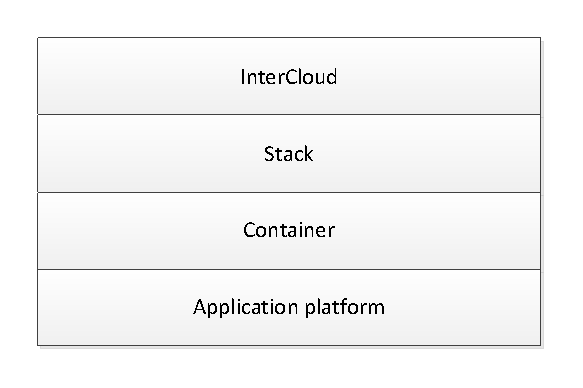
\includegraphics[width=0.5\textwidth]{chapter-5/sap-layers}
  \end{center}
  \caption{Layered structure of Cloud-SAP}
  \label{design:csap-layers}
\end{figure}

\subsection{Autonomic components}
Each layer of the Cloud-SAP (shown in figure \ref{design:csap-layers}) must be characterized by an ability to adapt to a given application usage. As the previous chapter stated, this can be achieved by adding an elasticity controller to each layer. This observation is a foundation of proposed architecture.

One of the first models that ensured system adaptivity is an autonomic component, concept based on a feed-back loop, initially proposed by IBM \cite{IBM06}. Figure \ref{ch5:autonomic-component} depicts that architecture. 

\begin{figure}[!ht]
  \begin{center}
    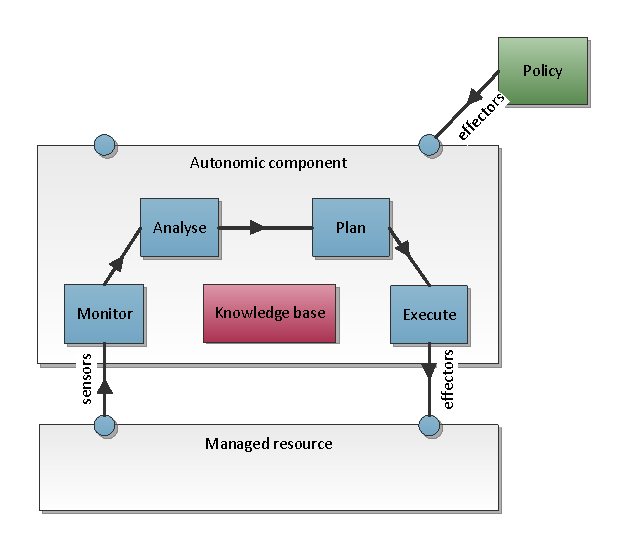
\includegraphics{chapter-5/autonomic-component}
  \end{center}
  \caption{autonomic component}
  \label{design:autonomic-component}
\end{figure}

Since designed platform operates on multiple layers, we can extend that model by using concept of a multi-hierarchical autonomic system \cite{LiWoZh05}. Figure \ref{ch5:hierarchical-autonomic-system} illustrates that hierarchy, were each level represents a different perspective on an application scaling. Using terminology characteristic to a autonomic system, first three hierarchy levels (application tuning, container, stack) are centralized and controlled by a single elasticity controller at each level, while the last inter-cloud level is a decentralized one - each cloud instance is fully independent.

As \cite{IBM06} states, each autonomic component has modules that are responsible for:
\begin{itemize}
	\item monitoring
	\item analysis
	\item planning
	\item action execution
\end{itemize}

While the managed component has:
\begin{itemize}
	\item sensors
	\item effectors
\end{itemize}

Due to the hierarchy of our architecture, each level manages an underlying autonomic component, while being managed by an upper layer at the very same time.
